\documentclass{article}
\usepackage{indentfirst}
\usepackage[utf8]{inputenc}
\usepackage[T1]{fontenc}
\usepackage[brazilian]{babel}
\usepackage{lmodern}
\usepackage{graphicx}
\usepackage{float}
\usepackage[]{subfigure}
\usepackage{afterpage}
\usepackage{amsmath}
\usepackage{textcomp,gensymb}
\usepackage{nameref}
\usepackage{accents}
\usepackage{listings}
\usepackage{color,soul}
\usepackage[margin=1in]{geometry}
\usepackage{steinmetz}

\PassOptionsToPackage{hyphens}{url}\usepackage{hyperref}
\hypersetup{
    breaklinks = true,
}
\urlstyle{same}
\newcommand{\ubar}[1]{\underaccent{\bar}{#1}}
%\renewcommand\thesection{\arabic{section}$^a$}
\renewcommand\thesection{\arabic{section}.}
\renewcommand\thesubsection{\arabic{section}.\alph{subsection}}
\definecolor{dkgreen}{rgb}{0,0.6,0}
\definecolor{gray}{rgb}{0.5,0.5,0.5}
\definecolor{mauve}{rgb}{0.58,0,0.82}
\lstset{
    frame=tb,
    language=Matlab,
    aboveskip=3mm,
    belowskip=3mm,
    showstringspaces=false,
    basicstyle={\small\ttfamily},
    numbers=none,
    numberstyle=\tiny\color{gray},
    keywordstyle=\color{blue},
    commentstyle=\color{dkgreen},
    stringstyle=\color{mauve},
    breaklines=true,
    breakatwhitespace=true,
    tabsize=4
}

\title{Simulação 3 - Controle Digital}
\author{Arthur de Matos Beggs - 12/0111098}
\date{2021}

\begin{document}
% capa
\begin{titlepage}
    \begin{center}
        \centering
        
\includegraphics[width=.7\linewidth]{images/logo_unb.png}\\[0.5cm]
        {\large \textbf{Universidade de Brasília}}\\[0.2cm]
        {\large \textbf{Departamento de Engenharia Elétrica}}\\[0.2cm]
        {\large \textbf{Controle Digital}}\\[4.8cm]
        {\bf \huge {Exercício de Simulação 3}}\\[0.2cm]
        {\bf \large {}}
    \end{center}

    \vspace{5cm}
    \hspace{2cm} {\noindent \bf \large {Aluno:}}\\
    \vspace{0.8cm}
    \hspace{2.35cm} {\large Arthur de Matos Beggs --------------------------------- 12/0111098}\\[1cm]

    \begin{center}
        {\large Brasília}\\
        {\large 2$^{\ubar{\circ}}$/2020}
    \end{center}

\end{titlepage}

\clearpage % Quebra de página

\setcounter{page}{2}


% \section{Questão 1}
%
%     \begin{figure}[H]
%        \centering
%             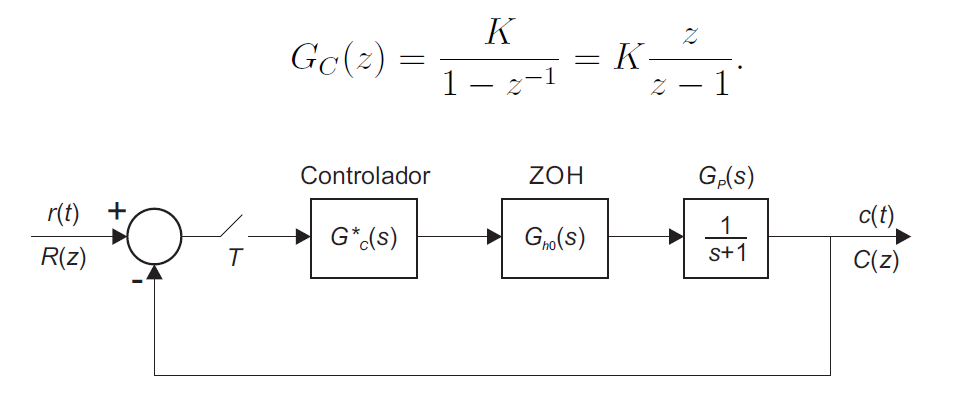
\includegraphics[width=1\linewidth]{images/Diagrama.png}
%             \caption{Diagrama e funções de transferência do sistema.}
%             \label{fig:diagram}
%     \end{figure}
%
%     {\textbf{a)} Para esboçar o LGR para os períodos de amostragem T = 0,5s, T = 1s e T = 2s, o seguinte script foi utilizado:}
%
% \vspace{7mm}
% \begin{lstlisting}
% s    = tf('s');
% Gp   = 1/(s+1);
%
% T1   = 0.5;
% z1   = tf('z',T1);
% Gc1  = z1/(z1-1);
% rl1  = c2d(Gp, T1, 'zoh') * Gc1;
%
% T2   = 1.0;
% z2   = tf('z',T2);
% Gc2  = z2/(z2-1);
% rl2  = c2d(Gp, T2, 'zoh') * Gc2;
%
% T3   = 2.0;
% z3   = tf('z',T3);
% Gc3  = z3/(z3-1);
% rl3  = c2d(Gp, T3, 'zoh') * Gc3;
%
% rlocus(rl1, rl2, rl3);
%
% \end{lstlisting}
%
%     \vspace{7mm}
%     {A execução do script gerou o \textit{plot} apresentado na Figura 2.}
%
%     \newpage
%
%     \begin{figure}[H]
%        \centering
%             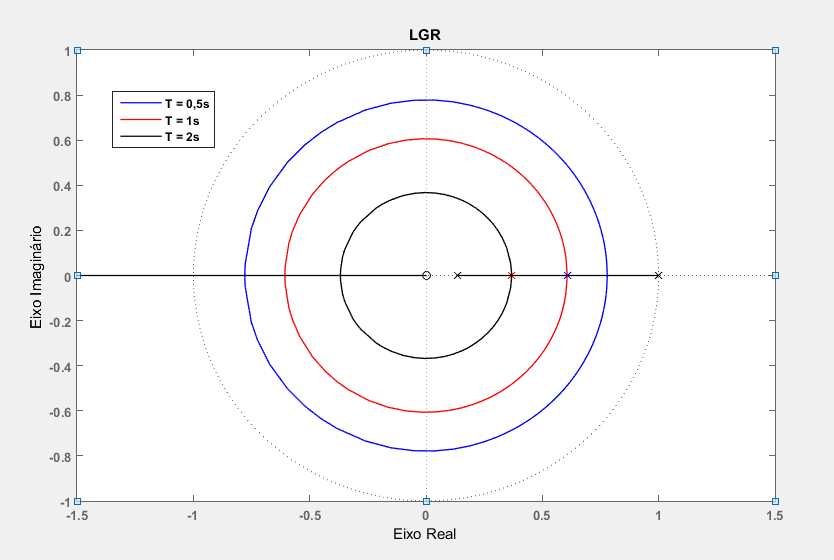
\includegraphics[width=1\linewidth]{images/LGR.png}
%             \caption{LGR no plano \textit{z} para T = 0,5s, 1s e 2s.}
%             \label{fig:lgr}
%     \end{figure}
%
%
%     \vspace{7mm}
%     {\textbf{b)} O valor de K crítico para cada período de amostragem é encontrado graficamente com o auxílio do cursor do Matlab no ponto em que o LGR deixa o círculo de raio unitário. A medida com o cursor apresenta uma imprecisão considerável, e por isso os valores de K crítico obtidos por esse método devem ser interpretados como aproximações.}
%
%     \vspace{7mm}
%     \begin{figure}[H]
%        \centering
%             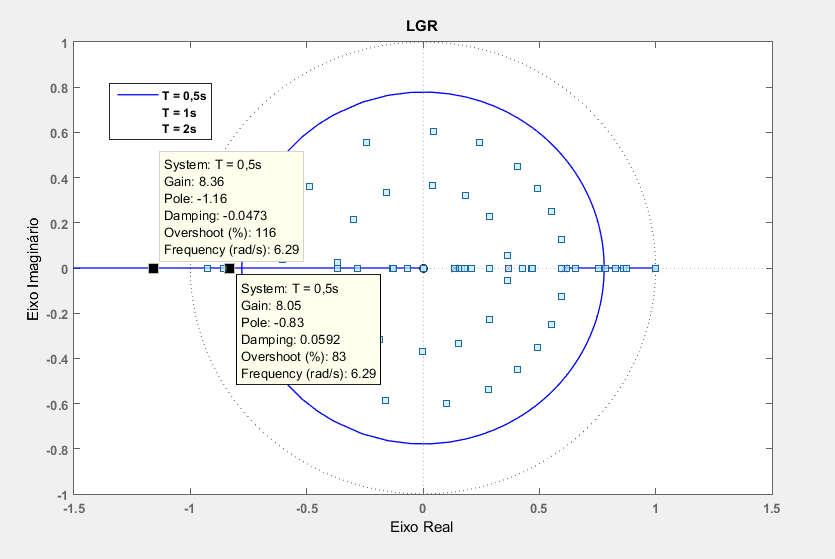
\includegraphics[width=.9\linewidth]{images/LGR_Kcrit05.png}
%             \caption{Para T = 0,5s, Kcrit $\approx$ 8,205 (obtido por interpolação).}
%             \label{fig:Kcrit05}
%     \end{figure}
%
%     \begin{figure}[H]
%        \centering
%             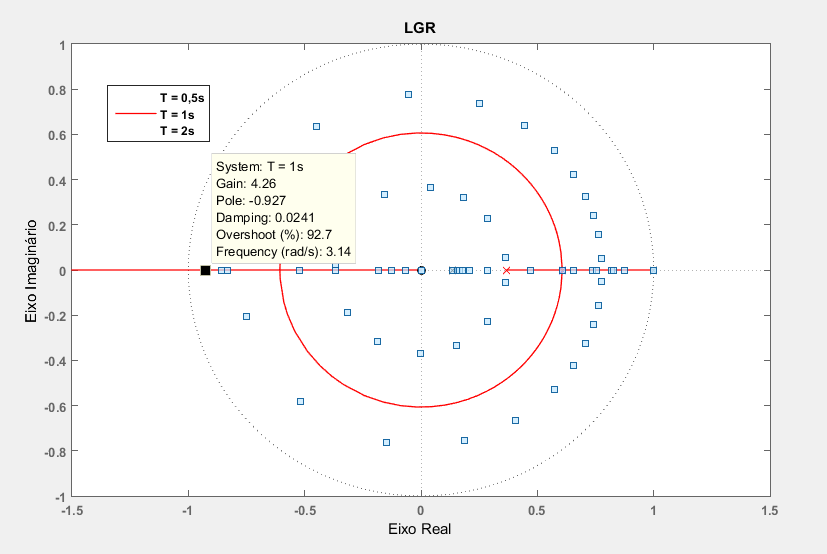
\includegraphics[width=1\linewidth]{images/LGR_Kcrit1.png}
%             \caption{Para T = 1s, Kcrit $\approx$ 4,26.}
%             \label{fig:Kcrit1}
%     \end{figure}
%
%     \begin{figure}[H]
%        \centering
%             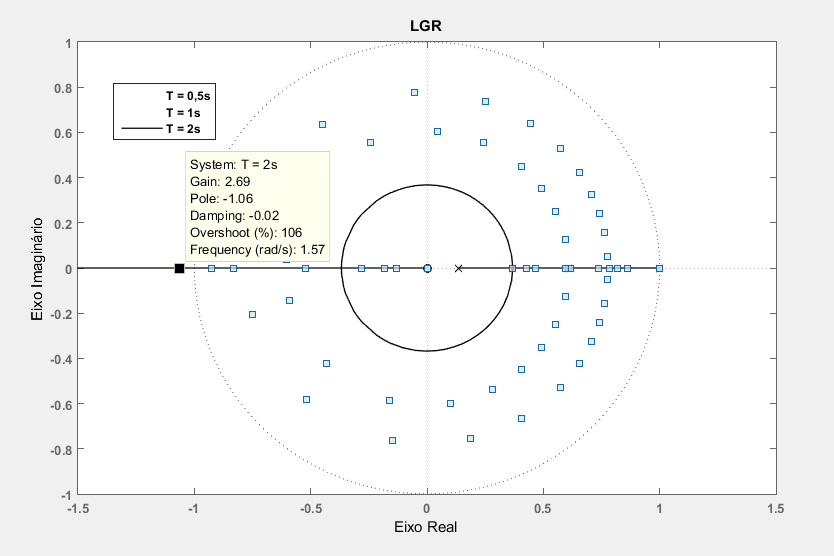
\includegraphics[width=1\linewidth]{images/LGR_Kcrit2.png}
%             \caption{Para T = 2s, Kcrit $\approx$ 2,69.}
%             \label{fig:Kcrit2}
%     \end{figure}
%
%     \clearpage
%
%     {\textbf{c)} Os pólos dominantes de malha fechada no plano \textit{z} quando K = 2 para cada valor de T foram obtidos posicionando o cursor sobre o ganho = 2. A medida com o cursor apresenta uma imprecisão considerável, e por isso os valores dos pólos dominantes obtidos por esse método devem ser interpretados como aproximações.}
%
%     \vspace{7mm}
%     \begin{figure}[H]
%        \centering
%             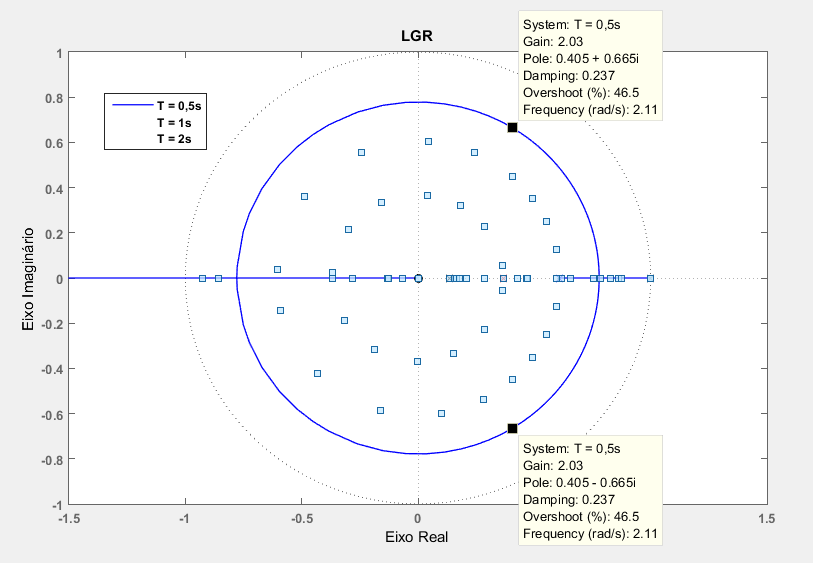
\includegraphics[width=.9\linewidth]{images/LGR_PoloDom05.png}
%             \caption{Para T = 0,5s, os pólos dominantes $\approx$ 0,405 $\pm$ 0,665j.}
%             \label{fig:poloDom05}
%     \end{figure}
%
%     \begin{figure}[H]
%        \centering
%             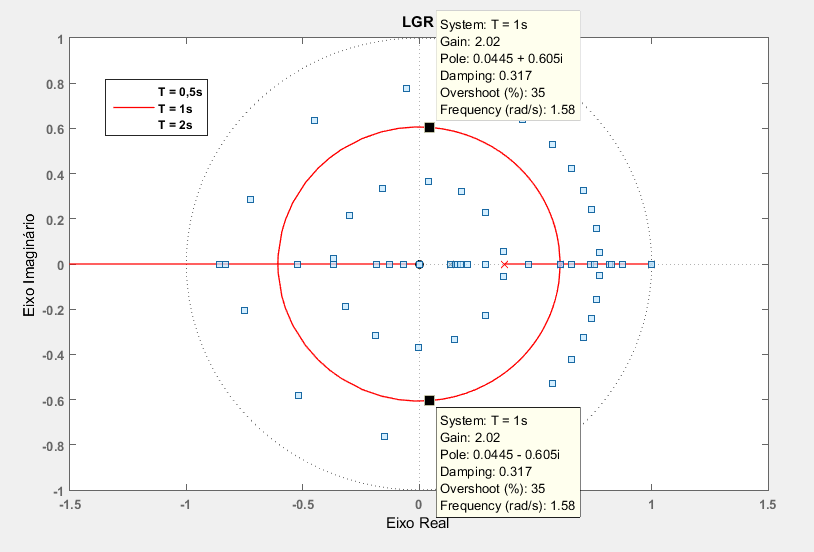
\includegraphics[width=.9\linewidth]{images/LGR_PoloDom1.png}
%             \caption{Para T = 1s, os pólos dominantes $\approx$ 0,0445 $\pm$ 0,605j.}
%             \label{fig:poloDom1}
%     \end{figure}
%
%     \begin{figure}[H]
%        \centering
%             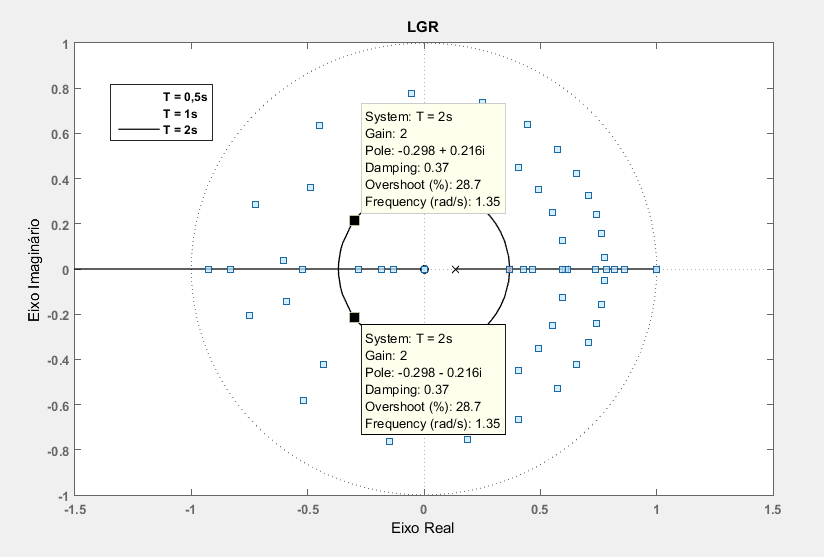
\includegraphics[width=1\linewidth]{images/LGR_PoloDom2.png}
%             \caption{Para T = 2s, os pólos dominantes $\approx$ -0,298 $\pm$ 0,216j.}
%             \label{fig:poloDom2}
%     \end{figure}
%
%
%     \vspace{7mm}
%     {Para as letras \textbf{d} e \textbf{e}, o diagrama do Simulink presente na Fig 9 foi utilizado.}
%
%     \begin{figure}[H]
%        \centering
%             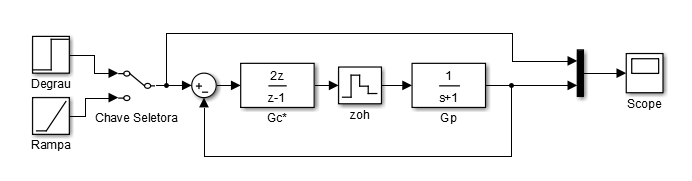
\includegraphics[width=1\linewidth]{images/DiagramaSimulink.png}
%             \caption{Diagrama do sistema representado no Simulink.}
%             \label{fig:diagSim}
%     \end{figure}
%
%     \vspace{14mm}
%     {\textbf{d)} As respostas ao degrau do sistema para diferentes tempos de amostragem e K = 2 são apresentadas nas figuras a seguir.}
%
%     \begin{figure}[H]
%        \centering
%             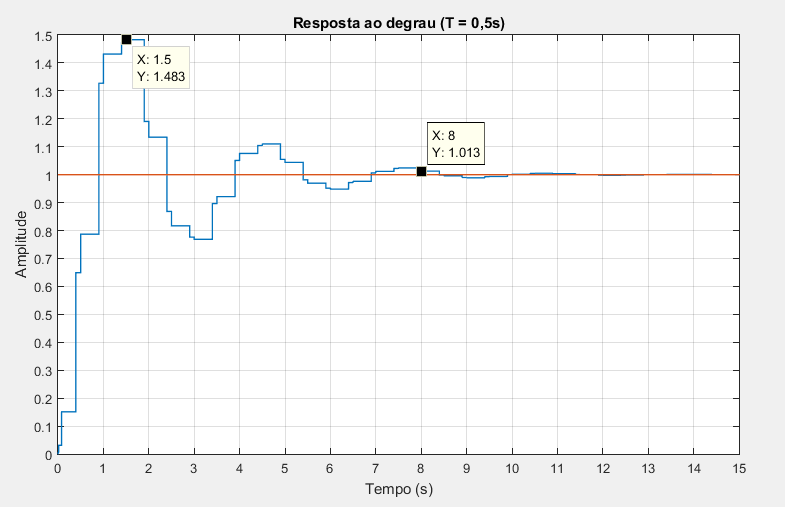
\includegraphics[width=1\linewidth]{images/rDeg05.png}
%             \caption{Resposta ao degrau unitário para T = 0,5s.}
%             \label{fig:rDeg05}
%     \end{figure}
%
%     {Para T = 0,5s, o sobressinal $\approx$  48,3\% e o tempo de acomodação $\approx$ 8 segundos.}
%
%     \vspace{7mm}
%     \begin{figure}[H]
%        \centering
%             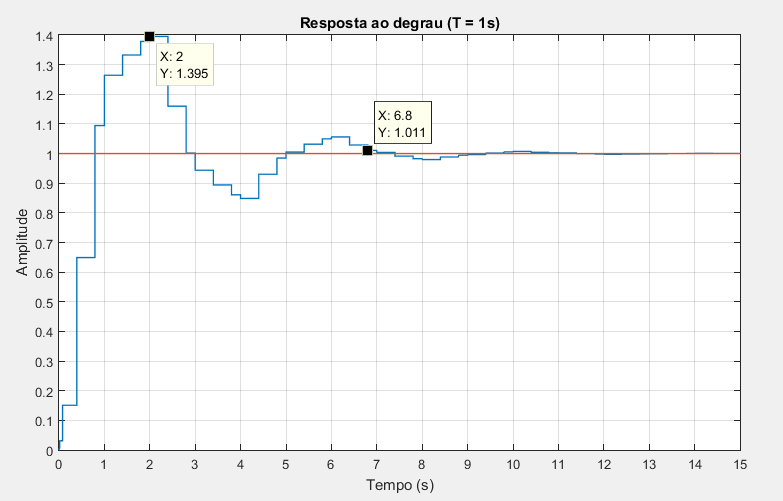
\includegraphics[width=1\linewidth]{images/rDeg1.png}
%             \caption{Resposta ao degrau unitário para T = 1s.}
%             \label{fig:rDeg1}
%     \end{figure}
%
%     {Para T = 1s, o sobressinal $\approx$ 39,5\% e o tempo de acomodação $\approx$ 6,8 segundos.}
%
%     \vspace{7mm}
%     \begin{figure}[H]
%        \centering
%             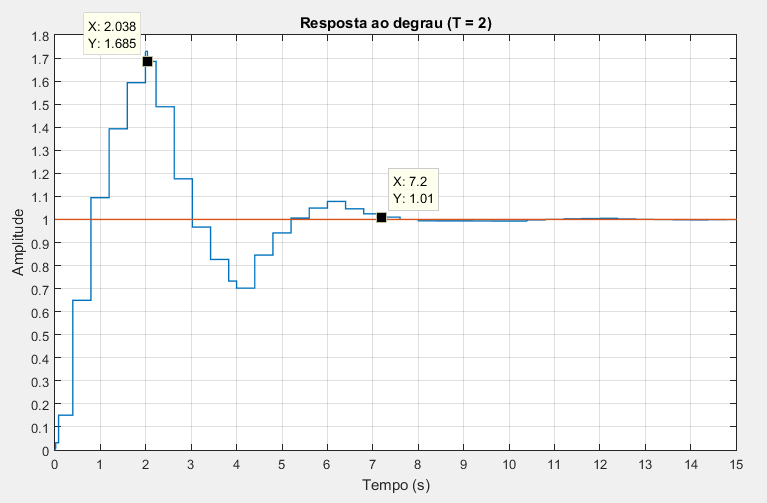
\includegraphics[width=1\linewidth]{images/rDeg2.png}
%             \caption{Resposta ao degrau unitário para T = 2s.}
%             \label{fig:rDeg2}
%     \end{figure}
%
%     {Para T = 2s, o sobressinal $\approx$ 68,5\% e o tempo de acomodação $\approx$ 7,2 segundos.}
%
%     \vspace{14mm}
%     {\textbf{e)} As respostas à rampa do sistema para diferentes tempos de amostragem e K = 2 são apresentadas nas figuras a seguir.}
%
%     \begin{figure}[H]
%        \centering
%             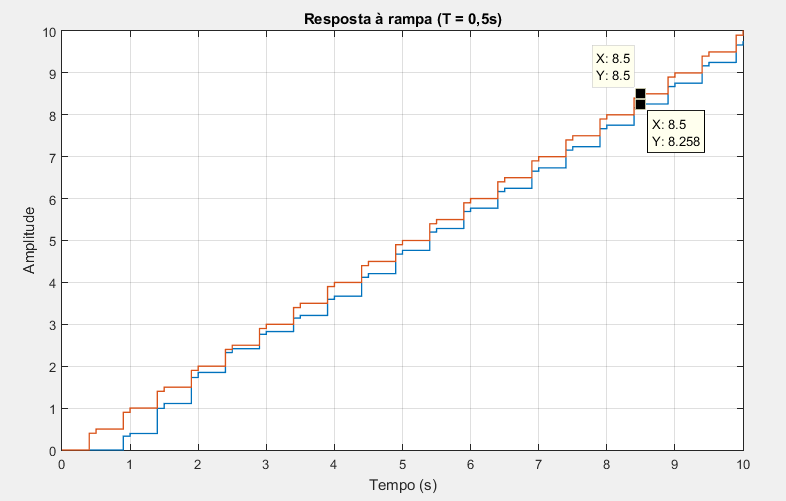
\includegraphics[width=1\linewidth]{images/rRamp05.png}
%             \caption{Resposta à rampa para T = 0,5s.}
%             \label{fig:rRamp05}
%     \end{figure}
%
%     {Para T = 0,5s, o erro em regime permanente Kv para uma entrada rampa $\approx$ 0,242.}
%
%     \vspace{7mm}
%     \begin{figure}[H]
%        \centering
%             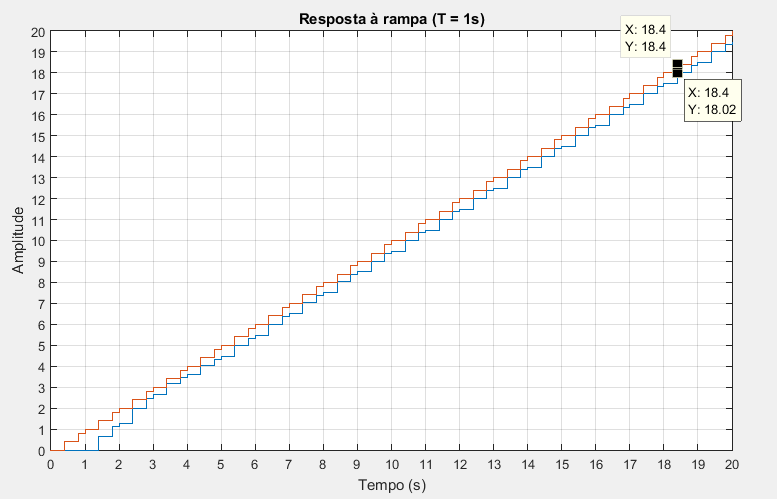
\includegraphics[width=1\linewidth]{images/rRamp1.png}
%             \caption{Resposta à rampa para T = 1s.}
%             \label{fig:rRamp1}
%     \end{figure}
%
%     {Para T = 1s, o erro em regime permanente Kv para uma entrada rampa $\approx$ 0,38.}
%
%     \vspace{7mm}
%     \begin{figure}[H]
%        \centering
%             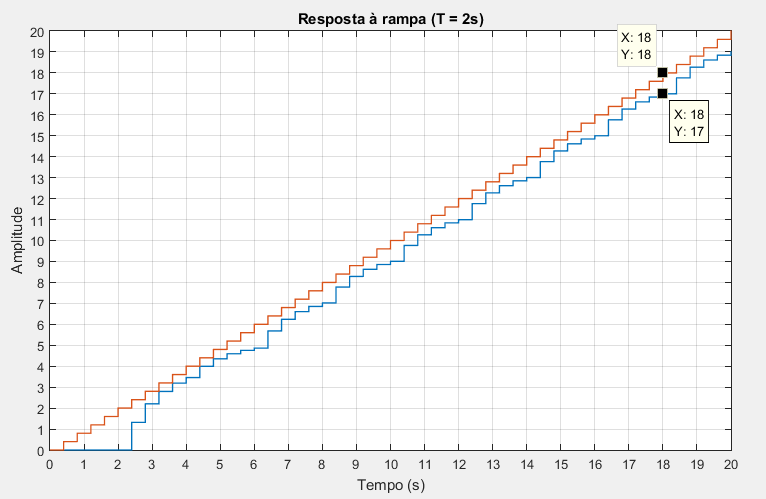
\includegraphics[width=1\linewidth]{images/rRamp2.png}
%             \caption{Resposta à rampa para T = 2s.}
%             \label{fig:rRamp2}
%     \end{figure}
%
%     {Para T = 2s, o erro em regime permanente Kv para uma entrada rampa $\approx$ 1.}
%
% %\newpage

%    \begin{figure}[H]
%       \centering
%            \includegraphics[width=1\linewidth]{images/.png}
%            \caption{}
%            \label{fig:}
%    \end{figure}

{\Large \bf Considere o sistema de controle a tempo discreto mostrado na
    Figura~\ref{fig:q2_diagrama}, cujo período de amostragem é $T = 0.2 s$.}

    \begin{figure}[H]
       \centering
            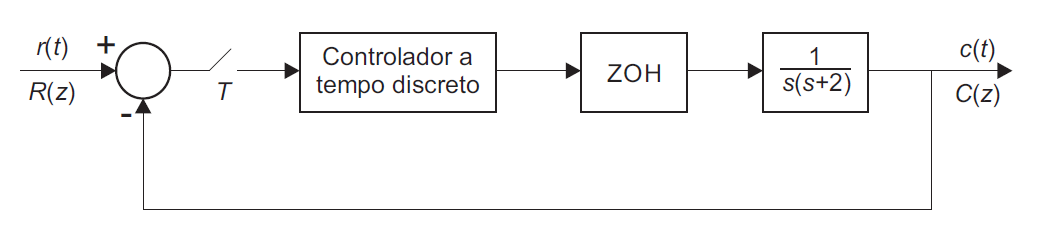
\includegraphics[width=1\linewidth]{images/q2_diagrama.png}
            \caption{Diagrama do sistema.}
            \label{fig:q2_diagrama}
    \end{figure}

    \section{Usando a técnica do LGR, projete no plano $z$ um controlador de
        modo que os polos dominantes de malha fechada tenham um fator de
        amortecimento $\zeta = 0.5$ e tempo de acomodação $t_s = 2\,s$:}

        \[ G_p(s) = G_{h0}(s) \times \frac{1}{s(s+2)} \]
        \[
            G_p(z) = \mathcal{Z}\left\{ G_{h0}(s) \times \frac{1}{s(s+2)} \right\}
                = (1-z^{-1}) \mathcal{Z}\left\{ \frac{1}{s^2 (s+2)} \right\}
        \]\\

        {Com o auxílio do Matlab,\\
        >> $T = 0.2;$\\
        >> $s = tf('s');$\\
        >> $z = tf('z', T);$\\
        >> $Gp\_s = zpk([\;], [0 \;\; -2], [1]);$\\
        >> $Gp\_z = c2d(Gp\_s, T, 'zoh')$ }\\

        \[ G_p(z) = \frac{0.01758(z+0.8753)}{(z-1)(z-0.6703)} \]\\

        {Temos que $t_s = \frac{4}{\zeta\omega_n}$, e dado que $t_s = 2\,s$ e
            $\zeta = 0.5$,}

        \[ \omega_n = \frac{4}{t_s\zeta} = 4 \,rad/s \]
        \[ \omega_d = \omega_n\sqrt{1-\zeta^2} = 3.4641 \,rad/s \]\\

        {Com $z = e^{sT} = e^{-\zeta\omega_nT}e^{j\omega_dT}$,}

        \[ |z| = e^{-\zeta\omega_nT} = 0.6703 \]
        \[ \angle z = \omega_dT = 39.6957^\circ \]\\

        {O par de polos complexos conjugados dominantes desejado pode ser
            encontrado por}

        \[ z_{dom} = |z|(\cos(\angle z) \pm j\sin(\angle z) = 0.5158 \pm j0.6387 \]\\

        {O LGR do sistema não controlado apresentado na Figura~\ref{fig:q2_lgr_descontrolado}
            foi obtido no Matlab usando os comandos\\
        >> $ hold \; on $\\
        >> $ rlocus(Gp\_z) $\\
        >> $ plot(real(z\_dom),imag(z\_dom),'r*',real(z\_dom),-imag(z\_dom),'r*') $ }\\

        \begin{figure}[H]
           \centering
                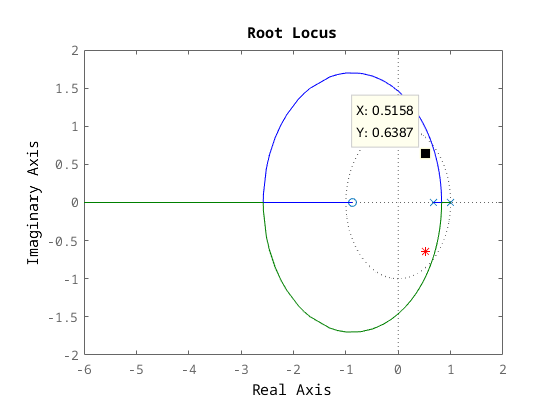
\includegraphics[width=1\linewidth]{images/q2_rlocus_uncontrolled.png}
                \caption{LGR do sistema $G_p(z)$, com os polos dominantes de
                    malha fechada representados por um asterisco vermelho e pelo
                    \textit{data cursor} do Matlab.}
                \label{fig:q2_lgr_descontrolado}
        \end{figure}

        {Pelo gráfico, o polo dominante desejado não faz parte do LGR do sistema.
            A condição de fase é utilizada para encontrar a contribuição angular
            que o controlador deve fornecer.}

        {O controlador projetado terá a forma $G_c(z) = K_c\frac{z - z_c}{z - p_c}$.

        {Como o a planta discretizada possui dois polos e um zero finito, o
            controlador fará o cancelamento do polo $z \neq 1$.}

        \[ \angle G_p(z) = \arctan\left( \frac{0.6387}{ 0.5158 + 0.8753 } \right)
                - \left(180^\circ - \arctan\left( \frac{0.6387}{ 1 - 0.5158 } \right) \right) \qquad\qquad\]
        \[\qquad\qquad\qquad\qquad - \left(180^\circ - \arctan\left( \frac{0.6387}{ 0.6703 - 0.5158 } \right) \right)
                + \left(180^\circ - \arctan\left( \frac{0.6387}{ 0.6703 - 0.5158 } \right) \right) \]\\
        \[ \angle G_p(z) = 102.5048^\circ \neq 180^\circ \pm 360^\circ i \]\\

        {Assim, o polo do controlador precisa contribuir com
        $180^\circ - 102.5048^\circ = 77.4951^\circ$.}

        \[ tan(77.4951^\circ) = \frac{0.6387}{ 0.5158 - p_c}
            \implies p_c = -\frac{0.6387}{tan(77.4951^\circ)} + 0.5158 = 0.3741 \]

        {O controlador projetado é dado por}
        \[ G_c(z) = K_c\frac{z - 0.6703}{z - 0.3741} \quad , \]
        {onde $K_c$ é o ganho do controlador.}

        {A função de transferência de malha aberta do sistema controlado é dada por}
        \[ G_s(z) = G_c(z) \times G_p(z) = \frac{0.01758K_c(z+0.8753)}{(z-1)(z-0.3741)} \]

        {O LGR do sistema $G_s(z)$ apresentado na Figura~\ref{fig:q2_lgr_controlled}
            foi obtido no Matlab usando os comandos\\
        >> $ hold \; on $\\
        >> $ Gs\_z = Gc\_z * Gp\_z $\\
        >> $ rlocus(Gs\_z) $\\
        >> $ plot(real(z\_dom),imag(z\_dom),'r*',real(z\_dom),-imag(z\_dom),'r*') $ }\\

        \begin{figure}[H]
           \centering
                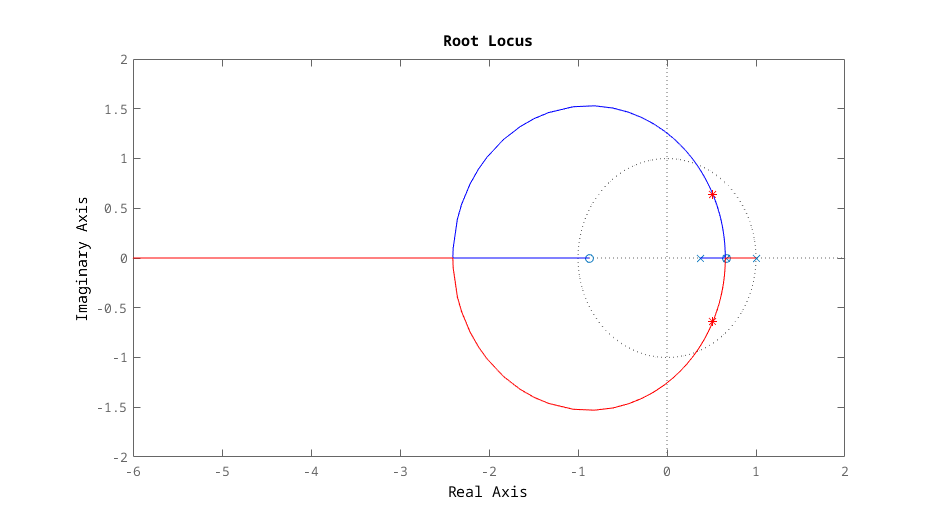
\includegraphics[width=1\linewidth]{images/q2_rlocus_controlled.png}
                \caption{LGR do sistema $G_s(z)$, com os polos dominantes de
                    malha fechada representados por asteriscos vermelhos
                    fazendo parte do LGR.}
                \label{fig:q2_lgr_controlled}
        \end{figure}

        {Para encontrar o ganho $K_c$ do controlador, a condição de módulo é
            utilizada. Assim,}
        \[ \left|G_s(z)|\right_{z= 0.5158 + j0.6387} = \frac{0.01758K_c \left|z + 0.8753|\right}{\left|z - 1|\right \left|z - 0.3741|\right} = 1 \]
        \[ \implies K_c = \left.\frac{\left|z - 1|\right \left|z - 0.3741|\right}{0.01758 \left|z + 0.8753|\right} \right|_{z= 0.5158 + j0.6387} = 19.4862 \]

        \[ G_c(z) = \frac{19.4862(z - 0.6703)}{(z - 0.3741)} \]



    \section{Obtenha computacionalmente a resposta ao degrau unitário do sistema
        em malha fechada. Verifique se os requisitos de projeto foram satisfeitos:}






    \section{Obtenha computacionalmente a resposta à rampa unitária do sistema
        em malha fechada. Determine o valor do erro estacionário:}





    \section{Refaça o projeto de modo que o valor do erro estacionário seja
        reduzido a um terço do valor anterior e fazendo o LGR passar próximo dos
        polos dominantes usados no item $(1)$. Obtenha computacionalmente a
        resposta à rampa unitária do sistema em malha fechada. Verifique se o
        requisito do erro estacionário foi atingido. Obtenha computacionalmente
        a resposta ao degrau unitário do sistema em malha fechada. A resposta
        transitória foi semelhante à do item $(1)$? Explique a diferença:}





\end{document}

